\documentclass[twoside]{book}

% Packages required by doxygen
\usepackage{fixltx2e}
\usepackage{calc}
\usepackage{doxygen}
\usepackage[export]{adjustbox} % also loads graphicx
\usepackage{graphicx}
\usepackage[utf8]{inputenc}
\usepackage{makeidx}
\usepackage{multicol}
\usepackage{multirow}
\PassOptionsToPackage{warn}{textcomp}
\usepackage{textcomp}
\usepackage[nointegrals]{wasysym}
\usepackage[table]{xcolor}

% Font selection
\usepackage[T1]{fontenc}
\usepackage[scaled=.90]{helvet}
\usepackage{courier}
\usepackage{amssymb}
\usepackage{sectsty}
\renewcommand{\familydefault}{\sfdefault}
\allsectionsfont{%
  \fontseries{bc}\selectfont%
  \color{darkgray}%
}
\renewcommand{\DoxyLabelFont}{%
  \fontseries{bc}\selectfont%
  \color{darkgray}%
}
\newcommand{\+}{\discretionary{\mbox{\scriptsize$\hookleftarrow$}}{}{}}

% Page & text layout
\usepackage{geometry}
\geometry{%
  a4paper,%
  top=2.5cm,%
  bottom=2.5cm,%
  left=2.5cm,%
  right=2.5cm%
}
\tolerance=750
\hfuzz=15pt
\hbadness=750
\setlength{\emergencystretch}{15pt}
\setlength{\parindent}{0cm}
\setlength{\parskip}{3ex plus 2ex minus 2ex}
\makeatletter
\renewcommand{\paragraph}{%
  \@startsection{paragraph}{4}{0ex}{-1.0ex}{1.0ex}{%
    \normalfont\normalsize\bfseries\SS@parafont%
  }%
}
\renewcommand{\subparagraph}{%
  \@startsection{subparagraph}{5}{0ex}{-1.0ex}{1.0ex}{%
    \normalfont\normalsize\bfseries\SS@subparafont%
  }%
}
\makeatother

% Headers & footers
\usepackage{fancyhdr}
\pagestyle{fancyplain}
\fancyhead[LE]{\fancyplain{}{\bfseries\thepage}}
\fancyhead[CE]{\fancyplain{}{}}
\fancyhead[RE]{\fancyplain{}{\bfseries\leftmark}}
\fancyhead[LO]{\fancyplain{}{\bfseries\rightmark}}
\fancyhead[CO]{\fancyplain{}{}}
\fancyhead[RO]{\fancyplain{}{\bfseries\thepage}}
\fancyfoot[LE]{\fancyplain{}{}}
\fancyfoot[CE]{\fancyplain{}{}}
\fancyfoot[RE]{\fancyplain{}{\bfseries\scriptsize Generated by Doxygen }}
\fancyfoot[LO]{\fancyplain{}{\bfseries\scriptsize Generated by Doxygen }}
\fancyfoot[CO]{\fancyplain{}{}}
\fancyfoot[RO]{\fancyplain{}{}}
\renewcommand{\footrulewidth}{0.4pt}
\renewcommand{\chaptermark}[1]{%
  \markboth{#1}{}%
}
\renewcommand{\sectionmark}[1]{%
  \markright{\thesection\ #1}%
}

% Indices & bibliography
\usepackage{natbib}
\usepackage[titles]{tocloft}
\setcounter{tocdepth}{3}
\setcounter{secnumdepth}{5}
\makeindex

% Hyperlinks (required, but should be loaded last)
\usepackage{ifpdf}
\ifpdf
  \usepackage[pdftex,pagebackref=true]{hyperref}
\else
  \usepackage[ps2pdf,pagebackref=true]{hyperref}
\fi
\hypersetup{%
  colorlinks=true,%
  linkcolor=blue,%
  citecolor=blue,%
  unicode%
}

% Custom commands
\newcommand{\clearemptydoublepage}{%
  \newpage{\pagestyle{empty}\cleardoublepage}%
}

\usepackage{caption}
\captionsetup{labelsep=space,justification=centering,font={bf},singlelinecheck=off,skip=4pt,position=top}

%===== C O N T E N T S =====

\begin{document}

% Titlepage & ToC
\hypersetup{pageanchor=false,
             bookmarksnumbered=true,
             pdfencoding=unicode
            }
\pagenumbering{roman}
\begin{titlepage}
\vspace*{7cm}
\begin{center}%
{\Large C\+AD }\\
\vspace*{1cm}
{\large Generated by Doxygen 1.8.11}\\
\end{center}
\end{titlepage}
\clearemptydoublepage
\tableofcontents
\clearemptydoublepage
\pagenumbering{arabic}
\hypersetup{pageanchor=true}

%--- Begin generated contents ---
\chapter{Class Index}
\section{Class List}
Here are the classes, structs, unions and interfaces with brief descriptions\+:\begin{DoxyCompactList}
\item\contentsline{section}{\hyperlink{structpoint2D}{point2D} \\*Points with 2 coordinates }{\pageref{structpoint2D}}{}
\item\contentsline{section}{\hyperlink{structpoint3D}{point3D} \\*Points with 3 coordinates }{\pageref{structpoint3D}}{}
\end{DoxyCompactList}

\chapter{File Index}
\section{File List}
Here is a list of all documented files with brief descriptions\+:\begin{DoxyCompactList}
\item\contentsline{section}{/home/mira/\+C\+Lion\+Projects/\+C\+A\+D/\hyperlink{graphics_8h}{graphics.\+h} \\*Functions for displaying 2D projections and 3D Model }{\pageref{graphics_8h}}{}
\item\contentsline{section}{/home/mira/\+C\+Lion\+Projects/\+C\+A\+D/\hyperlink{linalg_8h}{linalg.\+h} \\*Linear Algebraic Transformations using Eigen3 }{\pageref{linalg_8h}}{}
\item\contentsline{section}{/home/mira/\+C\+Lion\+Projects/\+C\+A\+D/\hyperlink{main_8cpp}{main.\+cpp} \\*Top-\/level driver code }{\pageref{main_8cpp}}{}
\item\contentsline{section}{/home/mira/\+C\+Lion\+Projects/\+C\+A\+D/\hyperlink{Point_8h}{Point.\+h} \\*Definitions of Point classes }{\pageref{Point_8h}}{}
\item\contentsline{section}{/home/mira/\+C\+Lion\+Projects/\+C\+A\+D/\hyperlink{util_8h}{util.\+h} \\*Utility Functions }{\pageref{util_8h}}{}
\end{DoxyCompactList}

\chapter{Class Documentation}
\hypertarget{structpoint2D}{}\section{point2D Struct Reference}
\label{structpoint2D}\index{point2D@{point2D}}


Points with 2 coordinates.  




{\ttfamily \#include $<$Point.\+h$>$}

\subsection*{Public Attributes}
\begin{DoxyCompactItemize}
\item 
double {\bfseries x}\hypertarget{structpoint2D_ade69032d2a9596dfd5c2b3ee29551569}{}\label{structpoint2D_ade69032d2a9596dfd5c2b3ee29551569}

\item 
double {\bfseries y}\hypertarget{structpoint2D_aeb2d0d7a7919611c9b6022fec6ca0bc6}{}\label{structpoint2D_aeb2d0d7a7919611c9b6022fec6ca0bc6}

\end{DoxyCompactItemize}


\subsection{Detailed Description}
Points with 2 coordinates. 

The documentation for this struct was generated from the following file\+:\begin{DoxyCompactItemize}
\item 
/home/mira/\+C\+Lion\+Projects/\+C\+A\+D/\hyperlink{Point_8h}{Point.\+h}\end{DoxyCompactItemize}

\hypertarget{structpoint3D}{}\section{point3D Struct Reference}
\label{structpoint3D}\index{point3D@{point3D}}


Points with 3 coordinates.  




{\ttfamily \#include $<$Point.\+h$>$}

\subsection*{Public Attributes}
\begin{DoxyCompactItemize}
\item 
double {\bfseries x}\hypertarget{structpoint3D_a931445a1beefab42e54ff84f200f53f3}{}\label{structpoint3D_a931445a1beefab42e54ff84f200f53f3}

\item 
double {\bfseries y}\hypertarget{structpoint3D_a78e4b9b1c38c7bec231e428f5c638153}{}\label{structpoint3D_a78e4b9b1c38c7bec231e428f5c638153}

\item 
double {\bfseries z}\hypertarget{structpoint3D_ae7370c9a05b6fb32d54c2b37a8b87d91}{}\label{structpoint3D_ae7370c9a05b6fb32d54c2b37a8b87d91}

\end{DoxyCompactItemize}


\subsection{Detailed Description}
Points with 3 coordinates. 

The documentation for this struct was generated from the following file\+:\begin{DoxyCompactItemize}
\item 
/home/mira/\+C\+Lion\+Projects/\+C\+A\+D/\hyperlink{Point_8h}{Point.\+h}\end{DoxyCompactItemize}

\chapter{File Documentation}
\hypertarget{graphics_8h}{}\section{/home/mira/\+C\+Lion\+Projects/\+C\+A\+D/graphics.h File Reference}
\label{graphics_8h}\index{/home/mira/\+C\+Lion\+Projects/\+C\+A\+D/graphics.\+h@{/home/mira/\+C\+Lion\+Projects/\+C\+A\+D/graphics.\+h}}


Functions for displaying 2D projections and 3D Model.  


{\ttfamily \#include $<$vector$>$}\\*
{\ttfamily \#include $<$G\+L/glut.\+h$>$}\\*
{\ttfamily \#include \char`\"{}Point.\+h\char`\"{}}\\*
Include dependency graph for graphics.\+h\+:\nopagebreak
\begin{figure}[H]
\begin{center}
\leavevmode
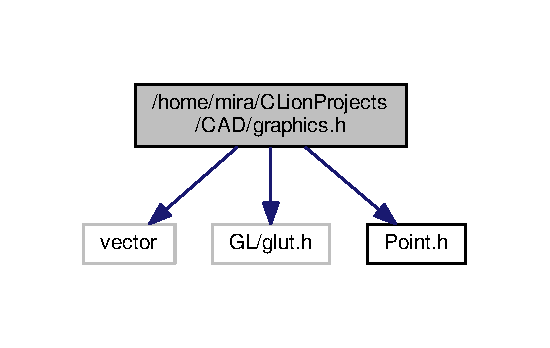
\includegraphics[width=264pt]{graphics_8h__incl}
\end{center}
\end{figure}
\subsection*{Functions}
\begin{DoxyCompactItemize}
\item 
void \hyperlink{graphics_8h_aa3f963682e4c9f411f3c9b509c53e7c9}{Display2\+D\+Proj} (vector$<$ \hyperlink{structpoint2D}{point2D} $>$ points, vector$<$ vector$<$ int $>$$>$ adj\+List)
\begin{DoxyCompactList}\small\item\em Display 2D projection. \end{DoxyCompactList}\item 
void \hyperlink{graphics_8h_a141648bb03759e0fb18d035fca6278ca}{Display3D} (vector$<$ \hyperlink{structpoint3D}{point3D} $>$ points, vector$<$ vector$<$ int $>$$>$ adj\+List)
\begin{DoxyCompactList}\small\item\em Display 3D model. \end{DoxyCompactList}\end{DoxyCompactItemize}


\subsection{Detailed Description}
Functions for displaying 2D projections and 3D Model. 

\begin{DoxyAuthor}{Author}
Mira Kabra 
\end{DoxyAuthor}
\begin{DoxyVersion}{Version}
1.\+0 
\end{DoxyVersion}
\begin{DoxyDate}{Date}
04-\/03-\/2018 
\end{DoxyDate}
\begin{DoxyNote}{Note}
The current proposed structure. Implementation yet to be started. 
\end{DoxyNote}


\subsection{Function Documentation}
\index{graphics.\+h@{graphics.\+h}!Display2\+D\+Proj@{Display2\+D\+Proj}}
\index{Display2\+D\+Proj@{Display2\+D\+Proj}!graphics.\+h@{graphics.\+h}}
\subsubsection[{\texorpdfstring{Display2\+D\+Proj(vector$<$ point2\+D $>$ points, vector$<$ vector$<$ int $>$$>$ adj\+List)}{Display2DProj(vector< point2D > points, vector< vector< int >> adjList)}}]{\setlength{\rightskip}{0pt plus 5cm}void Display2\+D\+Proj (
\begin{DoxyParamCaption}
\item[{vector$<$ {\bf point2D} $>$}]{points, }
\item[{vector$<$ vector$<$ int $>$$>$}]{adj\+List}
\end{DoxyParamCaption}
)}\hypertarget{graphics_8h_aa3f963682e4c9f411f3c9b509c53e7c9}{}\label{graphics_8h_aa3f963682e4c9f411f3c9b509c53e7c9}


Display 2D projection. 


\begin{DoxyParams}{Parameters}
{\em points} & list of 2D points \\
\hline
{\em adj\+List} & Shows the connectivity in terms of point number \\
\hline
\end{DoxyParams}
\index{graphics.\+h@{graphics.\+h}!Display3D@{Display3D}}
\index{Display3D@{Display3D}!graphics.\+h@{graphics.\+h}}
\subsubsection[{\texorpdfstring{Display3\+D(vector$<$ point3\+D $>$ points, vector$<$ vector$<$ int $>$$>$ adj\+List)}{Display3D(vector< point3D > points, vector< vector< int >> adjList)}}]{\setlength{\rightskip}{0pt plus 5cm}void Display3D (
\begin{DoxyParamCaption}
\item[{vector$<$ {\bf point3D} $>$}]{points, }
\item[{vector$<$ vector$<$ int $>$$>$}]{adj\+List}
\end{DoxyParamCaption}
)}\hypertarget{graphics_8h_a141648bb03759e0fb18d035fca6278ca}{}\label{graphics_8h_a141648bb03759e0fb18d035fca6278ca}


Display 3D model. 


\begin{DoxyParams}{Parameters}
{\em points} & list of 3D points \\
\hline
{\em adj\+List} & Shows connectivity in terms of point number \\
\hline
\end{DoxyParams}

\hypertarget{linalg_8h}{}\section{/home/mira/\+C\+Lion\+Projects/\+C\+A\+D/linalg.h File Reference}
\label{linalg_8h}\index{/home/mira/\+C\+Lion\+Projects/\+C\+A\+D/linalg.\+h@{/home/mira/\+C\+Lion\+Projects/\+C\+A\+D/linalg.\+h}}


Linear Algebraic Transformations using Eigen3.  


{\ttfamily \#include $<$vector$>$}\\*
{\ttfamily \#include $<$Eigen/\+Dense$>$}\\*
{\ttfamily \#include \char`\"{}Point.\+h\char`\"{}}\\*
Include dependency graph for linalg.\+h\+:\nopagebreak
\begin{figure}[H]
\begin{center}
\leavevmode
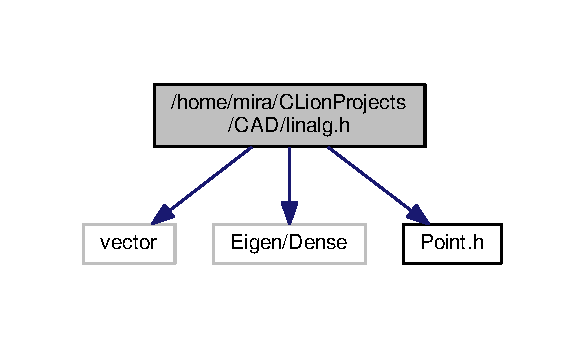
\includegraphics[width=281pt]{linalg_8h__incl}
\end{center}
\end{figure}
\subsection*{Functions}
\begin{DoxyCompactItemize}
\item 
vector$<$ \hyperlink{structpoint2D}{point2D} $>$ \hyperlink{linalg_8h_a65bebcda9de746fcb8f827b8200c371a}{Projection} (vector$<$ \hyperlink{structpoint3D}{point3D} $>$ points, \hyperlink{structpoint3D}{point3D} perpendicular)
\item 
vector$<$ \hyperlink{structpoint3D}{point3D} $>$ \hyperlink{linalg_8h_a7c4019b7a10749a52af8ce01e6b174b0}{Build3D} (vector$<$ \hyperlink{structpoint2D}{point2D} $>$ proj\+List1, vector$<$ \hyperlink{structpoint2D}{point2D} $>$ proj\+List2, \hyperlink{structpoint2D}{point2D} Ori1\mbox{[}3\mbox{]}, \hyperlink{structpoint2D}{point2D} Ori2\mbox{[}3\mbox{]})
\end{DoxyCompactItemize}


\subsection{Detailed Description}
Linear Algebraic Transformations using Eigen3. 

\begin{DoxyAuthor}{Author}
Mira Kabra 
\end{DoxyAuthor}
\begin{DoxyVersion}{Version}
1.\+0 
\end{DoxyVersion}
\begin{DoxyDate}{Date}
04-\/03-\/2018 
\end{DoxyDate}
\begin{DoxyNote}{Note}
The current proposed structure. Implementation yet to be started. 
\end{DoxyNote}


\subsection{Function Documentation}
\index{linalg.\+h@{linalg.\+h}!Build3D@{Build3D}}
\index{Build3D@{Build3D}!linalg.\+h@{linalg.\+h}}
\subsubsection[{\texorpdfstring{Build3\+D(vector$<$ point2\+D $>$ proj\+List1, vector$<$ point2\+D $>$ proj\+List2, point2\+D Ori1[3], point2\+D Ori2[3])}{Build3D(vector< point2D > projList1, vector< point2D > projList2, point2D Ori1[3], point2D Ori2[3])}}]{\setlength{\rightskip}{0pt plus 5cm}vector$<${\bf point3D}$>$ Build3D (
\begin{DoxyParamCaption}
\item[{vector$<$ {\bf point2D} $>$}]{proj\+List1, }
\item[{vector$<$ {\bf point2D} $>$}]{proj\+List2, }
\item[{{\bf point2D}}]{Ori1\mbox{[}3\mbox{]}, }
\item[{{\bf point2D}}]{Ori2\mbox{[}3\mbox{]}}
\end{DoxyParamCaption}
)}\hypertarget{linalg_8h_a7c4019b7a10749a52af8ce01e6b174b0}{}\label{linalg_8h_a7c4019b7a10749a52af8ce01e6b174b0}
For evaluating 3D points from the projected points on two different planes 
\begin{DoxyParams}{Parameters}
{\em set\+One} & list of 2D projections of points on to the first plane \\
\hline
{\em set\+Two} & list of 2D projections of points on to the second plane \\
\hline
{\em Ori1} & array containing projection of 3D points on the first plane \\
\hline
{\em Ori2} & array containing projection of 3D points on the second plane \\
\hline
\end{DoxyParams}
\begin{DoxyReturn}{Returns}
will return the evaluated 3D points corresponding to the projected points 
\end{DoxyReturn}
\index{linalg.\+h@{linalg.\+h}!Projection@{Projection}}
\index{Projection@{Projection}!linalg.\+h@{linalg.\+h}}
\subsubsection[{\texorpdfstring{Projection(vector$<$ point3\+D $>$ points, point3\+D perpendicular)}{Projection(vector< point3D > points, point3D perpendicular)}}]{\setlength{\rightskip}{0pt plus 5cm}vector$<${\bf point2D}$>$ Projection (
\begin{DoxyParamCaption}
\item[{vector$<$ {\bf point3D} $>$}]{points, }
\item[{{\bf point3D}}]{perpendicular}
\end{DoxyParamCaption}
)}\hypertarget{linalg_8h_a65bebcda9de746fcb8f827b8200c371a}{}\label{linalg_8h_a65bebcda9de746fcb8f827b8200c371a}
For evaluating the projection of 3D points on specified plane 
\begin{DoxyParams}{Parameters}
{\em points} & list of 3D points \\
\hline
{\em perpendicular} & perpendicular to the plane \\
\hline
\end{DoxyParams}
\begin{DoxyReturn}{Returns}
list of 2D projections of points on to the plane 
\end{DoxyReturn}

\hypertarget{main_8cpp}{}\section{/home/mira/\+C\+Lion\+Projects/\+C\+A\+D/main.cpp File Reference}
\label{main_8cpp}\index{/home/mira/\+C\+Lion\+Projects/\+C\+A\+D/main.\+cpp@{/home/mira/\+C\+Lion\+Projects/\+C\+A\+D/main.\+cpp}}


Top-\/level driver code.  


{\ttfamily \#include $<$iostream$>$}\\*
{\ttfamily \#include \char`\"{}Point.\+h\char`\"{}}\\*
{\ttfamily \#include \char`\"{}util.\+h\char`\"{}}\\*
Include dependency graph for main.\+cpp\+:
\nopagebreak
\begin{figure}[H]
\begin{center}
\leavevmode
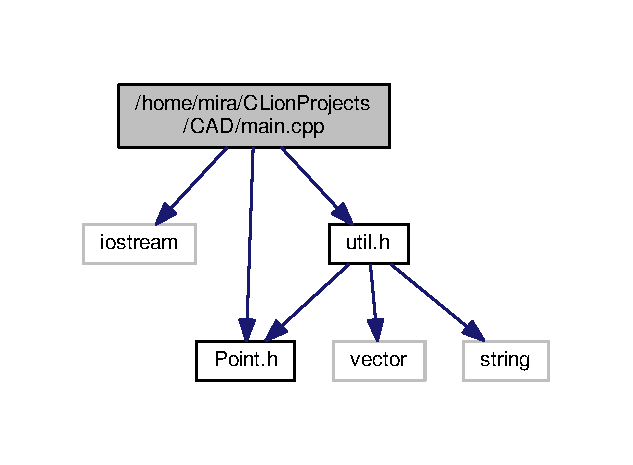
\includegraphics[width=304pt]{main_8cpp__incl}
\end{center}
\end{figure}
\subsection*{Functions}
\begin{DoxyCompactItemize}
\item 
int \hyperlink{main_8cpp_ae66f6b31b5ad750f1fe042a706a4e3d4}{main} ()
\end{DoxyCompactItemize}


\subsection{Detailed Description}
Top-\/level driver code. 

\begin{DoxyAuthor}{Author}
Mira Kabra 
\end{DoxyAuthor}
\begin{DoxyVersion}{Version}
1.\+0 
\end{DoxyVersion}
\begin{DoxyDate}{Date}
04-\/03-\/2018 
\end{DoxyDate}
\begin{DoxyNote}{Note}
The current proposed structure. Implementation yet to be started. 
\end{DoxyNote}


\subsection{Function Documentation}
\index{main.\+cpp@{main.\+cpp}!main@{main}}
\index{main@{main}!main.\+cpp@{main.\+cpp}}
\subsubsection[{\texorpdfstring{main()}{main()}}]{\setlength{\rightskip}{0pt plus 5cm}int main (
\begin{DoxyParamCaption}
{}
\end{DoxyParamCaption}
)}\hypertarget{main_8cpp_ae66f6b31b5ad750f1fe042a706a4e3d4}{}\label{main_8cpp_ae66f6b31b5ad750f1fe042a706a4e3d4}
Takes the mode information which specifies what function it needs to serve Takes the input files One with the coordinates and one with the edge information The edge input will be taken in the form of adjacency matrix whose data type will be \hyperlink{structpoint3D}{point3D} or \hyperlink{structpoint2D}{point2D} \begin{DoxyReturn}{Returns}

\end{DoxyReturn}

\hypertarget{Point_8h}{}\section{/home/mira/\+C\+Lion\+Projects/\+C\+A\+D/\+Point.h File Reference}
\label{Point_8h}\index{/home/mira/\+C\+Lion\+Projects/\+C\+A\+D/\+Point.\+h@{/home/mira/\+C\+Lion\+Projects/\+C\+A\+D/\+Point.\+h}}


Definitions of Point classes.  


This graph shows which files directly or indirectly include this file\+:
\nopagebreak
\begin{figure}[H]
\begin{center}
\leavevmode
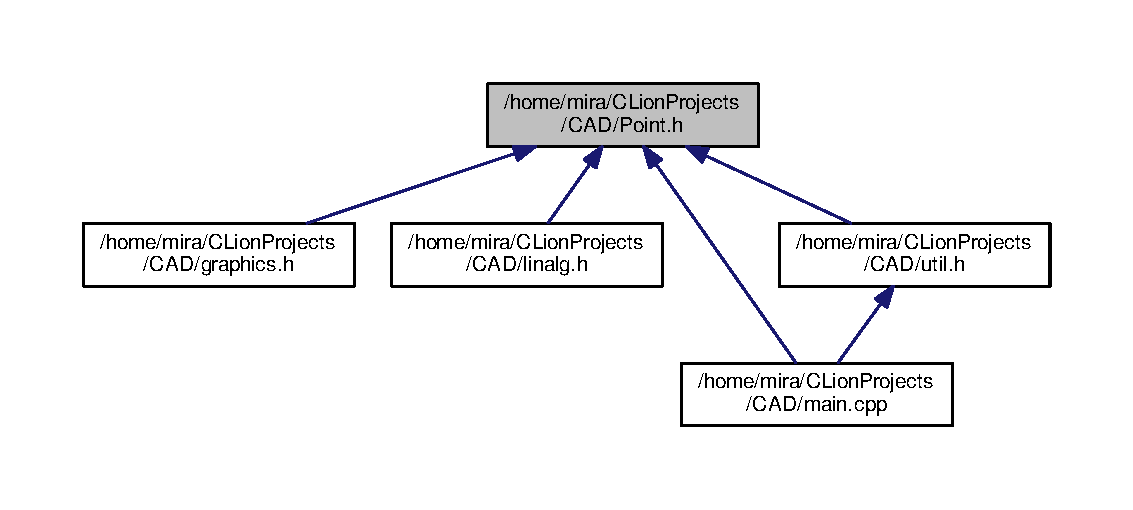
\includegraphics[width=350pt]{Point_8h__dep__incl}
\end{center}
\end{figure}
\subsection*{Classes}
\begin{DoxyCompactItemize}
\item 
struct \hyperlink{structpoint3D}{point3D}
\begin{DoxyCompactList}\small\item\em Points with 3 coordinates. \end{DoxyCompactList}\item 
struct \hyperlink{structpoint2D}{point2D}
\begin{DoxyCompactList}\small\item\em Points with 2 coordinates. \end{DoxyCompactList}\end{DoxyCompactItemize}


\subsection{Detailed Description}
Definitions of Point classes. 

\begin{DoxyAuthor}{Author}
Mira Kabra 
\end{DoxyAuthor}
\begin{DoxyVersion}{Version}
1.\+0 
\end{DoxyVersion}
\begin{DoxyDate}{Date}
04-\/03-\/2018 
\end{DoxyDate}
\begin{DoxyNote}{Note}
The current proposed structure. Implementation yet to be started. 
\end{DoxyNote}

\hypertarget{util_8h}{}\section{/home/mira/\+C\+Lion\+Projects/\+C\+A\+D/util.h File Reference}
\label{util_8h}\index{/home/mira/\+C\+Lion\+Projects/\+C\+A\+D/util.\+h@{/home/mira/\+C\+Lion\+Projects/\+C\+A\+D/util.\+h}}


Utility Functions.  


{\ttfamily \#include $<$vector$>$}\\*
{\ttfamily \#include $<$string$>$}\\*
{\ttfamily \#include \char`\"{}Point.\+h\char`\"{}}\\*
Include dependency graph for util.\+h\+:\nopagebreak
\begin{figure}[H]
\begin{center}
\leavevmode
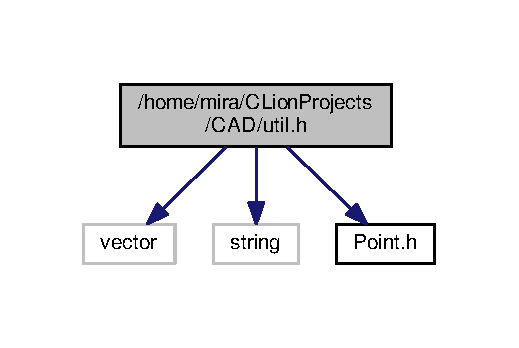
\includegraphics[width=249pt]{util_8h__incl}
\end{center}
\end{figure}
This graph shows which files directly or indirectly include this file\+:\nopagebreak
\begin{figure}[H]
\begin{center}
\leavevmode
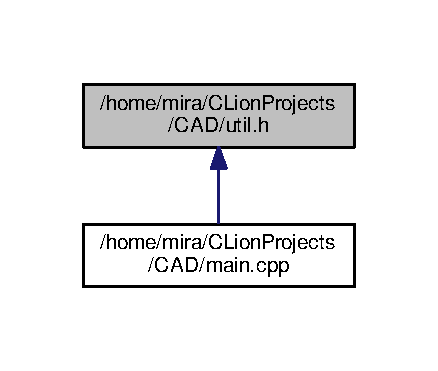
\includegraphics[width=210pt]{util_8h__dep__incl}
\end{center}
\end{figure}
\subsection*{Functions}
\begin{DoxyCompactItemize}
\item 
vector$<$ \hyperlink{structpoint2D}{point2D} $>$ \hyperlink{util_8h_a4eb7d175f2a2b97a360a255aa7679f7a}{read2\+D\+Proj} (string proj\+File\+Path)
\item 
vector$<$ \hyperlink{structpoint3D}{point3D} $>$ \hyperlink{util_8h_afe208903c2d009b7403516d6e6197a69}{read3\+D\+Model} (string model\+File\+Path)
\item 
vector$<$ vector$<$ int $>$ $>$ \hyperlink{util_8h_ad51698f50454d58d684de735b12556e5}{read\+Adjacency\+List} (string adj\+File\+Path)
\end{DoxyCompactItemize}


\subsection{Detailed Description}
Utility Functions. 

\begin{DoxyAuthor}{Author}
Mira Kabra 
\end{DoxyAuthor}
\begin{DoxyNote}{Note}
To be implemented. 
\end{DoxyNote}


\subsection{Function Documentation}
\index{util.\+h@{util.\+h}!read2\+D\+Proj@{read2\+D\+Proj}}
\index{read2\+D\+Proj@{read2\+D\+Proj}!util.\+h@{util.\+h}}
\subsubsection[{\texorpdfstring{read2\+D\+Proj(string proj\+File\+Path)}{read2DProj(string projFilePath)}}]{\setlength{\rightskip}{0pt plus 5cm}vector$<${\bf point2D}$>$ read2\+D\+Proj (
\begin{DoxyParamCaption}
\item[{string}]{proj\+File\+Path}
\end{DoxyParamCaption}
)}\hypertarget{util_8h_a4eb7d175f2a2b97a360a255aa7679f7a}{}\label{util_8h_a4eb7d175f2a2b97a360a255aa7679f7a}
Utility function for reading projection specification from given file. 
\begin{DoxyParams}{Parameters}
{\em proj\+File\+Path} & path to file containing projection specification \\
\hline
\end{DoxyParams}
\begin{DoxyReturn}{Returns}
List of 2D coordinates of points 
\end{DoxyReturn}
\index{util.\+h@{util.\+h}!read3\+D\+Model@{read3\+D\+Model}}
\index{read3\+D\+Model@{read3\+D\+Model}!util.\+h@{util.\+h}}
\subsubsection[{\texorpdfstring{read3\+D\+Model(string model\+File\+Path)}{read3DModel(string modelFilePath)}}]{\setlength{\rightskip}{0pt plus 5cm}vector$<${\bf point3D}$>$ read3\+D\+Model (
\begin{DoxyParamCaption}
\item[{string}]{model\+File\+Path}
\end{DoxyParamCaption}
)}\hypertarget{util_8h_afe208903c2d009b7403516d6e6197a69}{}\label{util_8h_afe208903c2d009b7403516d6e6197a69}
Utility function for reading 3D model specification from given file. 
\begin{DoxyParams}{Parameters}
{\em model\+File\+Path} & path to file containing projection specification \\
\hline
\end{DoxyParams}
\begin{DoxyReturn}{Returns}
List of 3D coordinates of points 
\end{DoxyReturn}
\index{util.\+h@{util.\+h}!read\+Adjacency\+List@{read\+Adjacency\+List}}
\index{read\+Adjacency\+List@{read\+Adjacency\+List}!util.\+h@{util.\+h}}
\subsubsection[{\texorpdfstring{read\+Adjacency\+List(string adj\+File\+Path)}{readAdjacencyList(string adjFilePath)}}]{\setlength{\rightskip}{0pt plus 5cm}vector$<$vector$<$int$>$ $>$ read\+Adjacency\+List (
\begin{DoxyParamCaption}
\item[{string}]{adj\+File\+Path}
\end{DoxyParamCaption}
)}\hypertarget{util_8h_ad51698f50454d58d684de735b12556e5}{}\label{util_8h_ad51698f50454d58d684de735b12556e5}
Utility function for reading adjacency list from given file. 
\begin{DoxyParams}{Parameters}
{\em adj\+File\+Path} & path to file containing projection specification \\
\hline
\end{DoxyParams}
\begin{DoxyReturn}{Returns}
adjacency list 
\end{DoxyReturn}

%--- End generated contents ---

% Index
\backmatter
\newpage
\phantomsection
\clearemptydoublepage
\addcontentsline{toc}{chapter}{Index}
\printindex

\end{document}
